\documentclass[conference]{IEEEtran}
\IEEEoverridecommandlockouts
% The preceding line is only needed to identify funding in the first footnote. If that is unneeded, please comment it out.
\usepackage{cite}
\usepackage{amsmath,amssymb,amsfonts}
\usepackage{algorithmic}
\usepackage{graphicx}
\usepackage{textcomp}
\usepackage{xcolor}

\usepackage{array}

\def\BibTeX{{\rm B\kern-.05em{\sc i\kern-.025em b}\kern-.08em
	T\kern-.1667em\lower.7ex\hbox{E}\kern-.125emX}}
	
\begin{document}

\title{Classification of Shark Behavior using K-Nearest Neigbours}

% \author{\IEEEauthorblockN{Sainesh Karan}
% 	\IEEEauthorblockA{\textit{Dept. of Electrical Engineering} \\
% 	\textit{California State University, Long Beach}\\
% 	Long Beach, USA}
% 	\and
% 	\IEEEauthorblockN{Emily Messe}
% 	\IEEEauthorblockA{\textit{Dept. of Biological Sciences} \\
% 	\textit{California State University, Long Beach}\\
% 	Long Beach, USA}
% 	\and
% 	\IEEEauthorblockN{Dr. Yu Yang}
% 	\IEEEauthorblockA{\textit{Dept. of Chemical Engineering} \\
% 	\textit{California State University, Long Beach}\\
% 	Long Beach, USA}
% 	\and
% 	\IEEEauthorblockN{Dr. Hen Guel Yeh}
% 	\IEEEauthorblockA{\textit{Dept. of Electrical Engineering} \\
% 	\textit{California State University, Long Beach}\\
% 	Long Beach, USA}
% 	\and
% 	\IEEEauthorblockN{Dr. Chris Lowe}
% 	\IEEEauthorblockA{\textit{Dept. of Biological Sciences} \\
% 	\textit{California State University, Long Beach}\\
% 	Long Beach, USA}
% 	\and
% 	\IEEEauthorblockN{Dr. Wenlu Zhang}
% 	\IEEEauthorblockA{\textit{Dept. of Computer Science} \\
% 	\textit{California State University, Long Beach}\\
% 	Long Beach, USA}
% }

% \author{
% 	\IEEEauthorblockN{Sainesh Karan\IEEEauthorrefmark{1}, Emily Messe\IEEEauthorrefmark{2}, Dr. Yu Yang\IEEEauthorrefmark{3}, Dr.Hen-Guel Yeh\IEEEauthorrefmark{1}, Dr. Chris Lowe\IEEEauthorrefmark{2}, Dr. Wenlu Zhang\IEEEauthorrefmark{4}}
% 	\IEEEauthorblockA{\IEEEauthorrefmark{1}\textit{Dept. of Electrical Engineering, California State University, Long Beach, CA - 90840}\\
% \IEEEauthorrefmark{2}\textit{Dept. of Biological Sciences, California State University, Long Beach, CA- 90840\\
% \IEEEauthorrefmark{3}\textit{Dept. of Chemical Engineering, California State University, Long Beach, CA- 90840\\}
% \IEEEauthorrefmark{4}\textit{Dept. of Computer Science,California State University, Long Beach, CA- 90840\newline}
% }}}

\author{
	\IEEEauthorblockN{Sainesh Karan\IEEEauthorrefmark{1}, Emily Messe\IEEEauthorrefmark{2}, Dr. Yu Yang\IEEEauthorrefmark{3}, Dr.Hen-Guel Yeh\IEEEauthorrefmark{1}, Dr. Chris Lowe\IEEEauthorrefmark{2}, Dr. Wenlu Zhang\IEEEauthorrefmark{4}}
	\IEEEauthorblockA{\IEEEauthorrefmark{1}Dept. of Electrical Engineering, California State University, Long Beach, CA - 90840}
	\IEEEauthorblockA{\IEEEauthorrefmark{2}Dept. of Biological Sciences, California State University, Long Beach, CA - 90840}
	\IEEEauthorblockA{\IEEEauthorrefmark{3}Dept. of Chemical Engineering, California State University, Long Beach, CA - 90840}
	\IEEEauthorblockA{\IEEEauthorrefmark{4}Dept. of Computer Science, California State University, Long Beach, CA - 90840}
}

\maketitle

\begin{abstract}
In this paper, we aim to ascertain the behavior of California Horn sharks (Heterodontus francisci) based on accelerometer data using a machine learning algorithm called Nearest Neighbors. We use digital signal processing techniques such as Fast Fourier Transform (FFT) and Discrete Cosine Transform (DCT) to represent the accelerometer signal in the frequency domain which reduces the data size required for training the classifier, the computation time and the memory resources needed, in addition to improving model accuracy. The shark behavior is classified into four classes namely Resting, Swimming, Feeding and Non-Directed Motion. We compare different combinations of time and frequency domain data on the performance of the algorithm. It is shown that the transform domain data considerably improved the accuracy of the classifier.
\end{abstract}

\begin{IEEEkeywords}
Activity Recognition, Shark Behavior, KNN, Digital Signal Processing, Machine Learning
\end{IEEEkeywords}

% squeeze figures vertically
\section{Introduction}
Activity recognition pertains to the task of classifying physical activities undertaken by an individual from the collected data. Differentiating behaviors of free-ranging animals provides an insight into their feeding patterns that help us understand their ecology and their impact on the environment. Recently, accelerometers have been employed to unveil the abstruse lives of marine animals.   It is extremely arduous to observe such species in their natural environments over long periods due to poor visibility, deeper depths, and adverse environmental conditions \cite{1}. Over the years bio-telemetry devices have become popular amongst researchers to overcome these obstacles and are widely available. An Acceleration Data Logger (ADL) is one such device that measures acceleration caused by body movements that can be used to determine body orientation and kinematics for behavioral classification \cite{1}. ADLs allow data to be recorded and stored at high frequencies, and thus providing high-resolution data with useful information to reveal the animal’s behavior. However, the increased   volume of high-resolution data is non-trivial to process, and the useful information hidden behind may not be easy to extract. This challenge motivates the research of automatic behavioral classification by using machine learning techniques.

The past few years have seen tremendous development in the fields of machine learning and artificial intelligence, which has spurred a widespread adoption of the technology for several applications. Machine learning algorithms can be broadly categorized into supervised and unsupervised methods. In supervised methods, a training data-set, which consists of the data and the associated outcome/labels, is used to train a model to accurately map the input variables to the outcome/labels. Once the model has been built based on the training data, it can be used to make predictions on new input data. Examples of such algorithms include Decision Trees, Random Forest (RF), K-Nearest Neighbors (KNN) and Neural Networks \cite{1}. 
Several studies have been conducted in the past to study the behavior of free-ranging animals using data loggers and machine learning techniques. In  \cite{2} and  \cite{3}, the authors demonstrate the utility of using data loggers and machine learning algorithms to classify the behavior of Griffon vultures and Cheetahs, respectively. In  \cite{4} authors used machine learning techniques to identify the hunting and feeding pattern of penguins. Apart from behavior classification, authors of  \cite{5} and  \cite{6} have used data loggers to determine the mortality and energy expenditure of sharks, respectively.

In this paper, we apply the KNN algorithm to classify data collected from the ADL into four behavior classes namely Resting, Swimming, Feeding, and Non-directed motion. KNN is a simple machine learning algorithm in which, a new data point is classified based on the majority of its $k$ nearest neighbors, $k$ being a user defined hyper-parameter. The algorithm does not use any model to fit the new data sample but rather computes the distance of the data point form its neighbors  \cite{7}. We also explore the effect of signal transformation techniques such as Discrete Fourier Transform (DFT) and Discrete Cosine Transform (DCT) on the performance of the classification algorithm. We expect that the transformation techniques will enhance the differentiating features of each behavior class thereby aiding the algorithm in the process while reducing the computation complexity and time. All data pre-processing, simulations and machine learning techniques used in this paper were implemented in Matlab R2018b® using the Statistics and Machine Learning Tool Box Ver.11.4.

\section{Data Aquisition and Pre-Processing}

\subsection{Data Aquisition}
Laboratory trials were conducted to quantify acceleration signatures of California horn sharks (Heterodontus francisci) for different behaviors including resting, swimming, and feeding (prey capture and handling). Horn sharks were chosen as a model species to represent a demersal, resting shark that are capable of eating hard-shelled invertebrates \cite{8, 9, 10}. Sharks were collected from Santa Catalina Island, and transported back to the CSULB Shark Lab. Trials occurred with a single shark in a 340L tank with two GoPro video cameras, one mounted on the bottom of the tank, and one above the tank. For each trial, a shark was fitted with an accelerometer data logger (ADL; Cefas G6a+ or Technosmart AxyDepth) via a custom tag package. Accelerometers recorded 3D acceleration data at 25 Hz. All acceleration data was processed in IgorPro (vers. 6.2, WaveMetrics) using Ethographer \cite{11}. Static acceleration represents the 3D body position and orientation due to gravity (i.e., pitch, X static; roll, Y static; yaw, Z static), whereas dynamic acceleration represents the 3D body movements (i.e., surge, X dynamic; heave, Y dynamic; sway, Z dynamic) as shown in Figure 1. Static acceleration was separated from dynamic acceleration using a 2 second box smoother \cite{12}. The plots for the raw data from Dataset 6 are shown in Figures 2 and 3; the plots represent the tri-axial Static and Dynamic data collected from the trial that was conducted between 5:39 and 6:56pm. Sharks were tagged approximately 6 hours before the start of the trial to allow the shark to acclimate. 

To characterize motion patterns associated with prey manipulation and handling, instrumented sharks were then fed three different prey types including a live purple urchin ($< 4$ cm test diameter), a frozen and thawed squid (whole, with pen), and a frozen and thawed shrimp. Prey was buried or placed away from the shark in order to characterize natural feeding behaviors expected in the field. A trial concluded when the shark had consumed all trial prey. Trials were approximately 2 hours long, and a total of seven trials were done on four different individuals. 

\begin{figure}[h]
	\centering
	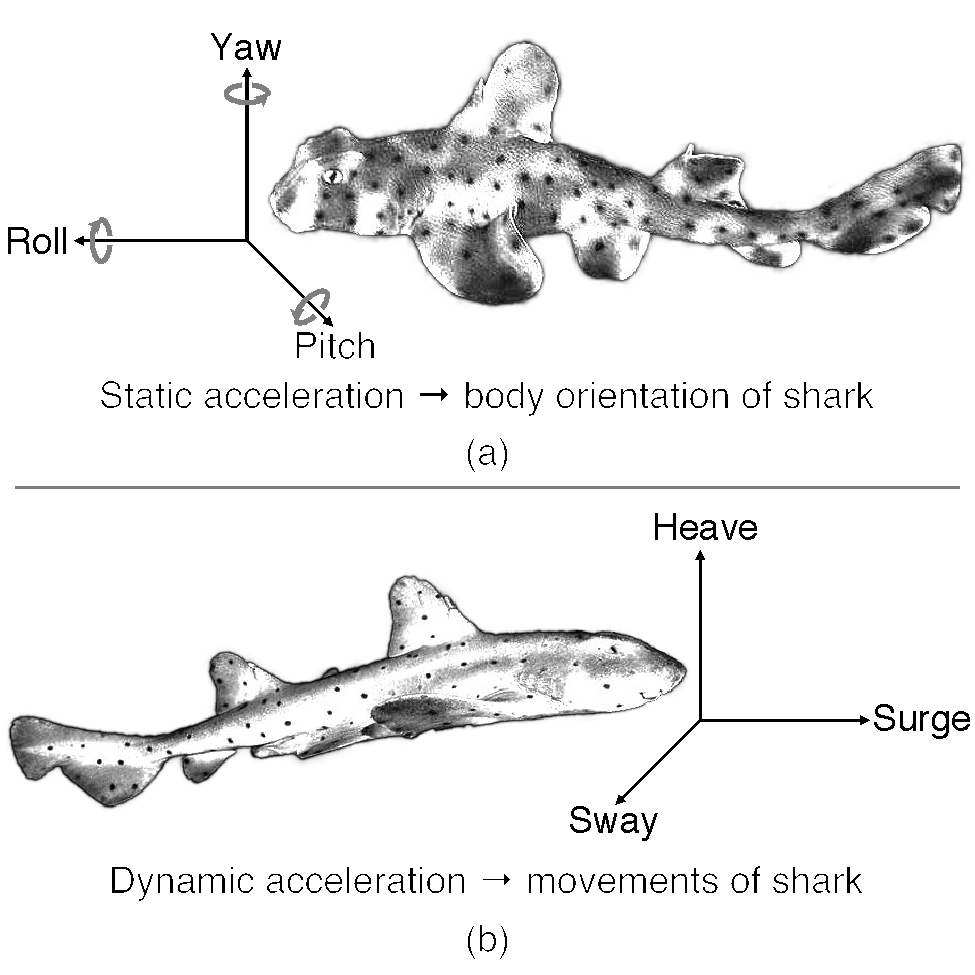
\includegraphics[width=3.49in]{accel.pdf}
	\caption{Breakdown of tri-axial acceleration data. (a) Static acceleration represents the body position and orientation      of the shark due to gravity. (b) Dynamic acceleration represents the body movements of the shark.}
	\label{accel}
\end{figure} % add markers for the time

The data generated by the ADL was labelled manually by viewing the GoPro video recording of each trial and identifying the shark behaviour with the corresponding time-stamps. All data samples that were unlabelled were removed from the dataset. 
\begin{figure}[h]
	\centering
	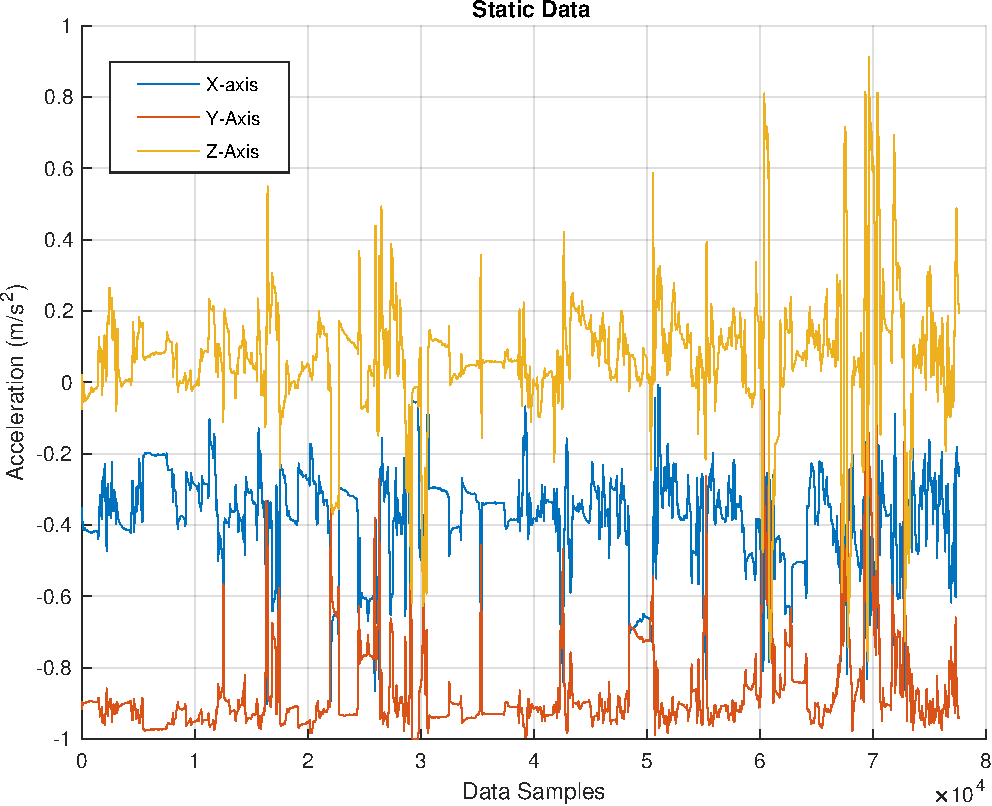
\includegraphics[width=3.49in]{1_static.pdf}
	\caption{The plots represent Static tri-axial data collected at 25 Hz for a period of approximately 2 hours.}
	\label{static}
\end{figure}
\begin{figure}[h]
	\centering
	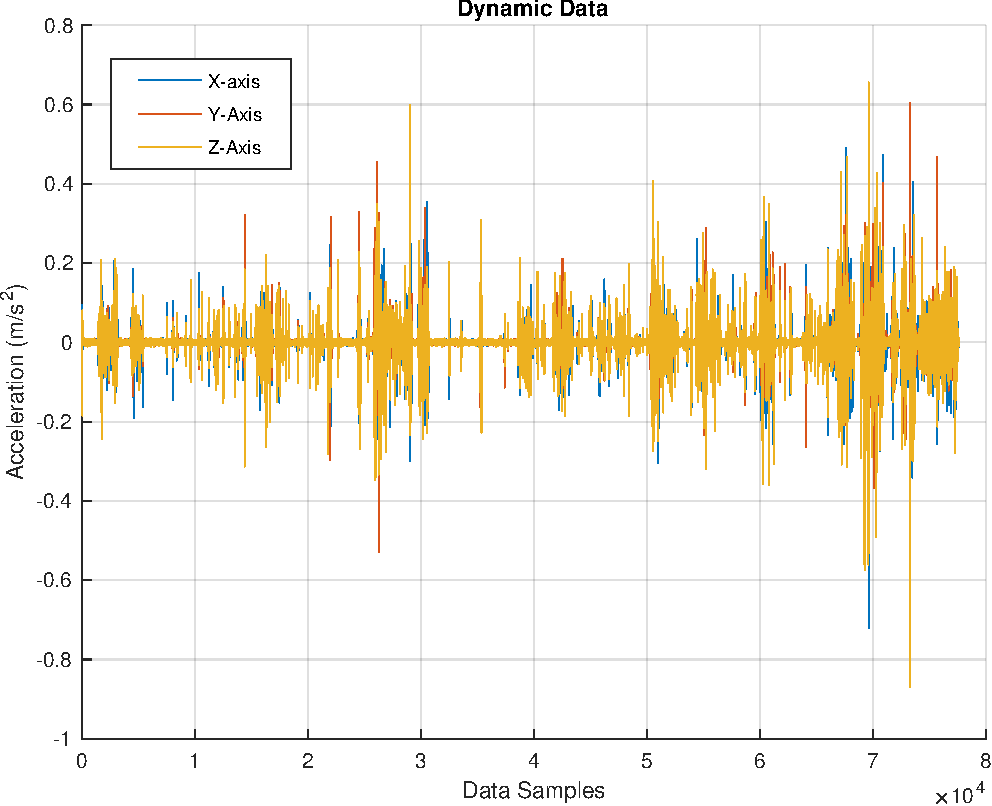
\includegraphics[width=3.49in]{2_dynamic.pdf}
	\caption{The plots represent Dynamic tri-axial data collected at 25 Hz for a period of approximately 2 hours.}
	\label{dynamic}
\end{figure}

\subsection{Data Pre-processing}
A total of seven datasets were formed from the trials. Each dataset was then separated into its four constituent behaviour classes based on the labels. The distribution of different classes in each dataset is presented in table 1. Because the datasets had very few feeding samples in comparison to other classes, carefull consideration had to be given to how the data is split between training and testing. In our scheme, Dataset 5 was chosen as the test data in order to maximize the number of feeding samples in the training data while still having enough feeding samples to test the model.  In addition, Dataset 5 came from a different individual shark as compared to other datasets, which allows us to examine the generalization capability of the classifier.
Next we combined all the datasets and subtracted the mean from all the data samples in the combined dataset so as to remove the DC-bias and noise, and centering the signal around zero. 
As can be seen from Table 1, the trials were of varying lengths with varying distribution of classes. As a result, the datasets were found to be biased with respect to the feeding behavior with the total Feeding samples being an order of magnitude lower than that of the other classes. In order to overcome this bias, we chose a subset of data samples from each of the remaining classes that was most consistent and free of noise. A total of 100,000 samples were chosen for Resting behavior with similarly equal samples taken from each dataset; 90,000 samples were chosen for swimming and 83,900 samples for Non-directed motion, respectively. The distribution of the chosen subsets is presented in Table II.
\begin{table*}[tp!]
	\centering
	\caption{Distribution of different behavior classes in the datasets}
	\begin{tabular}{l r r r r r r r r}
	\hline
	& \textbf{Dataset 1} & \textbf{Dataset 2} & \textbf{Dataset 3} & \textbf{Dataset 4} & \textbf{Dataset 5} & \textbf{Dataset 6} & \textbf{Dataset 7} & \multicolumn{1}{c}{\textbf{Total}}\\
	\hline
	Resting & 157,750 & 565,580 & 379,850 & 10,250 & 6,150 & 27,975 & 77,374 & 1,224,929 \\
	Swimming & 6,200 & 209,550 & 5,100 & 81,525 & 7,975 & 19,750 & 61,475 & 391575 \\
	Feeding & 5,700 & 350 & 200 & 1,375 & 875 & 2,900 & 2,100 & 13,500 \\
	NDM & 51,950 & 7,400 & 15,700 & 1,750 & 1,775 & 27,025 & 5,400 & 11,1000 \\
	Total & 22,1600 & 782,880 & 40,0850 & 94,900 & 16,775 & 77,650 & 146,349 & -- \\
	\hline
	\end{tabular}
	\label{}
\end{table*}

\begin{table*}[tp!]
	\centering
	\caption{Class distribution of chosen subsets used for training}
	\begin{tabular}{l r r r r r r r}
	\hline
	& \textbf{Dataset 1} & \textbf{Dataset 2} & \textbf{Dataset 3} & \textbf{Dataset 5} & \textbf{Dataset 6} & \textbf{Dataset 7} & \multicolumn{1}{c}{\textbf{Total}}\\
	\hline
	Resting & 20,000 & 20,000 & 20,000 & 10,000 & 15,000 & 15,000 & 100,000 \\
	Swimming & 6,000 & 20,000 & 5,000 & 20,000 & 19,000 & 20,000 & 90,000 \\
	Feeding & 5,700 & 350 & 200 & 1,375 & 2,900 & 2,100 & 12,625 \\
	NDM & 30,000 & 7,000 & 15,000 & 1,500 & 25,000 & 5,400 & 83,900 \\
	Total & 61,700 & 47,350 & 40,200 & 32,875 & 62,900 & 42,500 & -- \\
	\hline
	\end{tabular}
	\label{}
\end{table*}
To improve the classifier efficiency, we convert the input signals into different domains of representation. Transforming signals into frequency domain allows us to capture the repetitive nature of the signals \cite{13}. This repetition often correlates to the periodic nature of a specific activity such as the tail beat of the shark while swimming or movement of the head while feeding.  Among the most popularly used transformation techniques is the Fourier Transform, which allows one to represent the most important characteristics of a time-based signal such as its  DC and dominant frequency components in the frequency domain as shown in Figures 4 and 5 for the collective Feeding data. Fast Fourier Transform (FFT) decomposes an input signal into its constituent sinusoids. In addition to the FFT, other frequency-based representations have been used such as Discrete Cosine Transform (DCT) which in contrast, decomposes a given signal into its constituent cosine waves. DCT returns an ordered sequence of coefficients such that the most significant information is concentrated at the lower indices of the sequence as can be seen from Figures 6 and 7.  This means that higher DCT coefficients can be discarded without losing information, which makes DCT suitable for data compression \cite{14}.
\begin{figure}[h!]
	\centering
	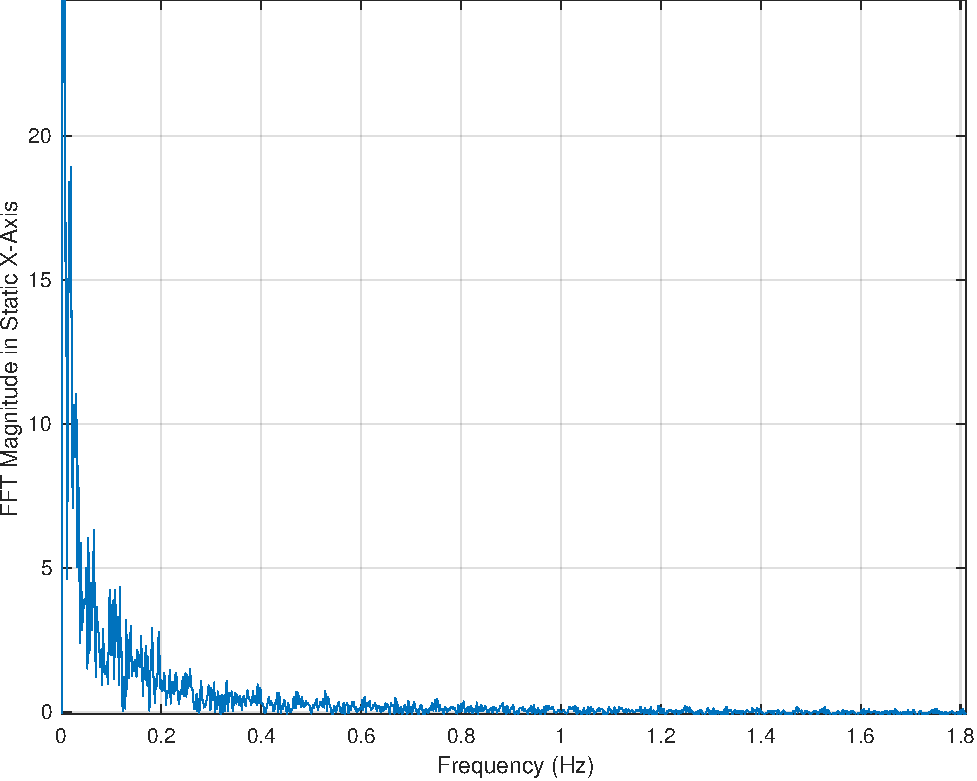
\includegraphics[width=3.1in]{3_feed_static_fft.pdf}
	\caption{The plot represents the Fourier Transform of Static X -axis of the collective Feeding data from Datasets 1-7 }
	\label{dynamic}
\end{figure}
\begin{figure}[h!]
	\centering
	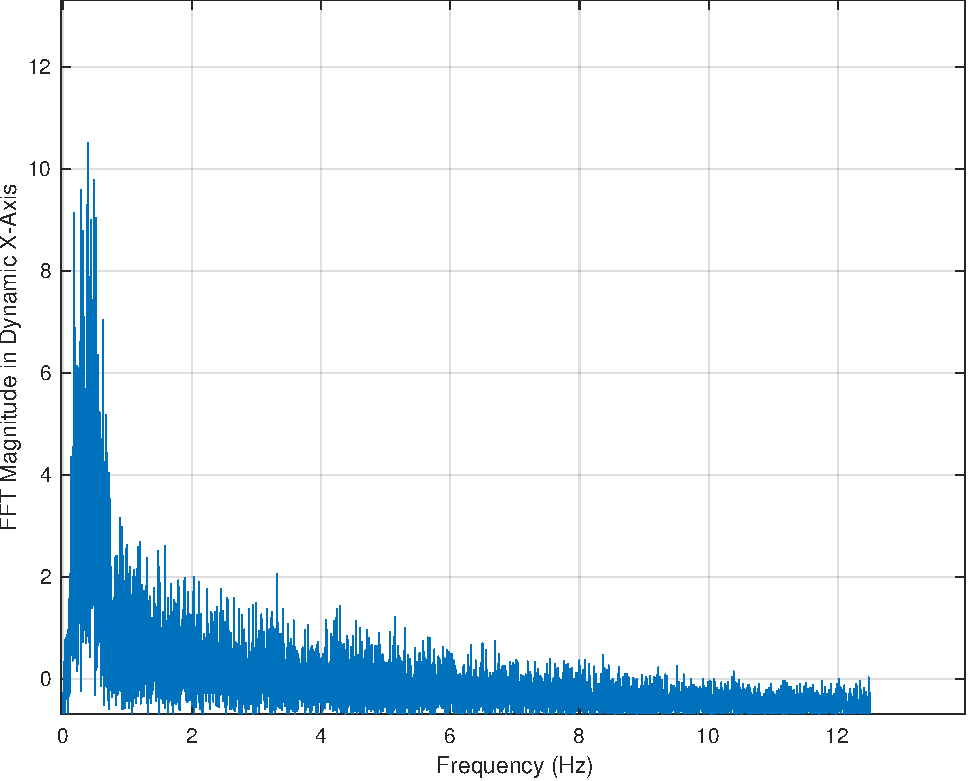
\includegraphics[width=3.1in]{4_feed_dynamic_fft.pdf}
	\caption{The plot represents the Fourier Transform of Dynamic X -axis of the collective Feeding data from Datasets 1-7}
	\label{dynamic}
\end{figure}
\begin{figure}[h!]
	\centering
	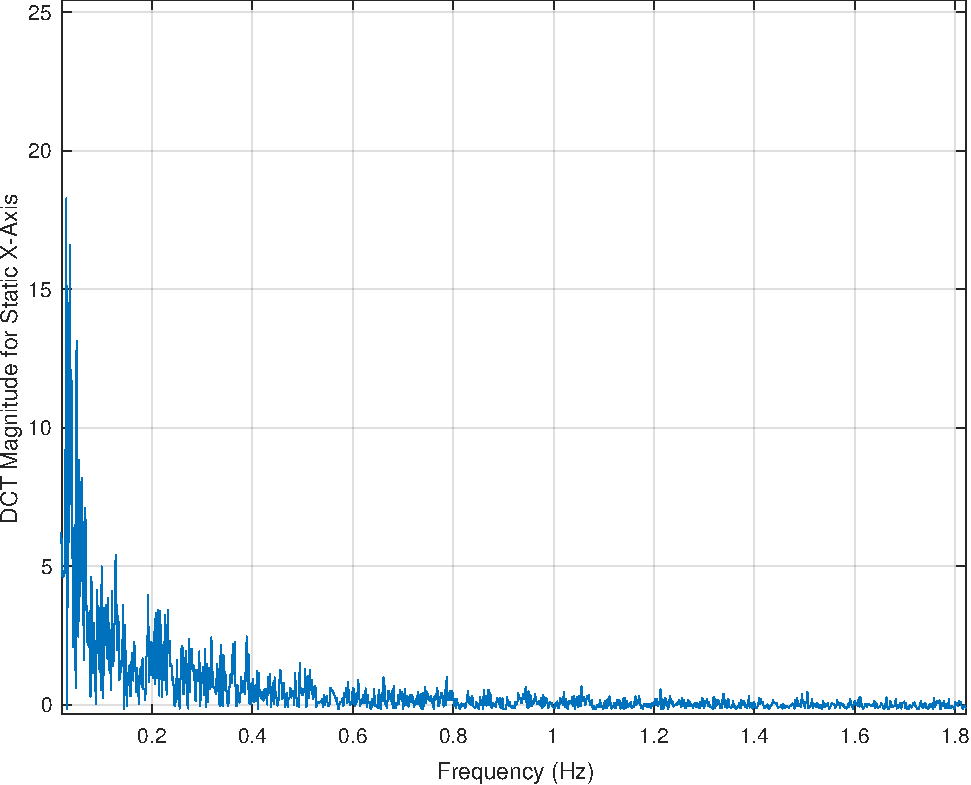
\includegraphics[width=3.1in]{5_feed_static_dct.pdf}
	\caption{The plot represents the Discrete Cosine Transform of Static X -axis of the collective Feeding data from Datasets 1-7}
	\label{dynamic}
\end{figure}
\begin{figure}[h!]
	\centering
	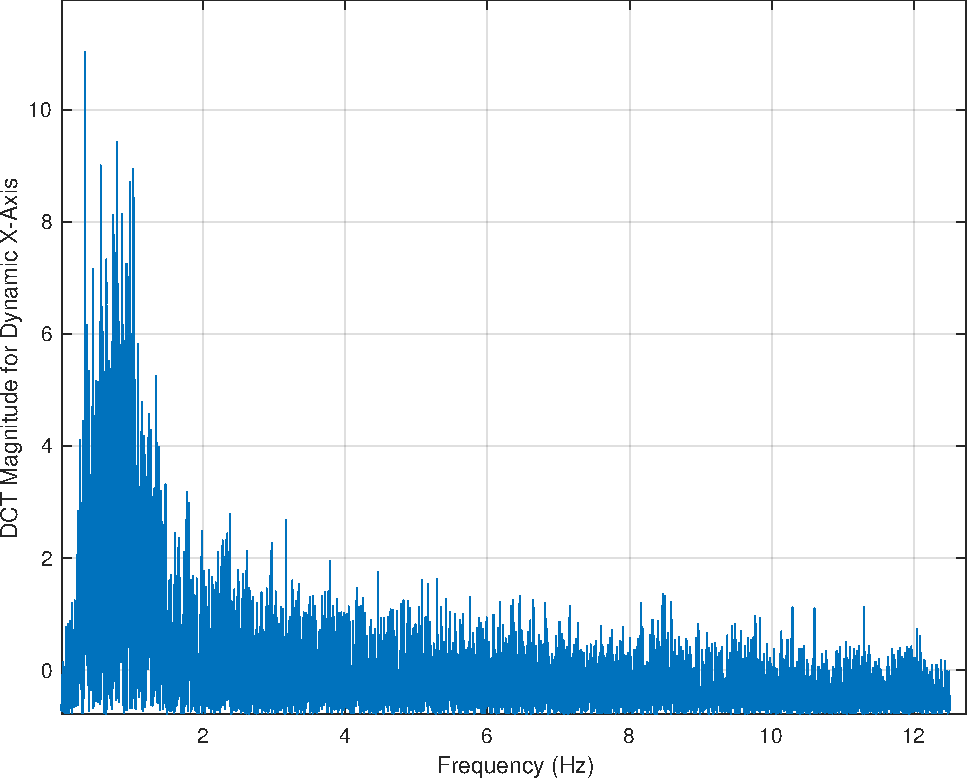
\includegraphics[width=3.1in]{6_feed_dynamic_dct.pdf}
	\caption{The plot represents the Discrete Cosine Transform of Dynamic X -axis of the collective Feeding data from Datasets 1-7}
	\label{dynamic}
\end{figure}
We compute the frequency analysis for the time signal of a specific length or window using the Fast Fourier Transform (FFT) algorithm. In this case we use a window of 25 data samples or 1 second so as to match the sampling frequency of the ADL and to avoid the transitioning of behaviour classes within the window. In order to overcome the bias in the training dataset against feeding class. We oversampled the feeding data by sliding the window with a 50\% overlap \cite{15} so as increase the number of feeding samples in the training dataset. Due to the symmetric property of Fourier Transform, we use only the 50\% of the data in the frequency domain. Similarly, we use only 50\% of the data of the DCT and discard the data in the higher frequency bins. However, it should be noted that the data reduction take place in when we use the transform domain data by itself. In the event where we combine the time and frequency domain data, the complete FFT and DCT are used so as to keep the input matrix to the model consistent. In such cases, no data reduction takes place. The total data samples in the transform domain are shown in Table III.
Thus by considering only the half of the Fourier transform i.e. ignoring the mirror image and the high frequency components of the DCT, we can reduce the total size of the data to be classified by half.
\begin{table}[h] % need to wrap
	\centering
	\caption{Total data samples in the transform domain used for training the model.}
	\begin{tabular}{p{0.65in} >{\raggedleft\arraybackslash}m{0.69in} >{\raggedleft\arraybackslash}m{0.69in} >{\raggedleft\arraybackslash}m{0.69in}}
	\hline
	\multicolumn{1}{>{\centering\arraybackslash}m{0.65in}}{\textbf{Behavior class}} &  \multicolumn{1}{>{\centering\arraybackslash}m{0.69in}}{\textbf{Data samples, time domain}} & \multicolumn{1}{>{\centering\arraybackslash}m{0.69in}}{\textbf{Data samples, transform domain}} & \multicolumn{1}{>{\centering\arraybackslash}m{0.69in}}{\textbf{Data reduction representation}}\\
	\hline
	Resting	& 100,000& 48,000	& 2.083 \\
	Swimming& 90,000 & 43,200	& 2.083 \\
	Feeding	& 12,625 & 6,060 	& 2.083 \\
	NDM		& 83,900 & 40,270	& 2.083 \\
	\hline
	\end{tabular}
	\label{total samples}
\end{table}

\section{Behavior Classification using K-Nearest Neighbors}
K-Nearest Neighbor is a supervised learning algorithm where the result of new test sample is classified based on the majority of its $k$ nearest neighbors, where $k$ is a user defined hyper-parameter. The neighbors are determined by measuring the distance between the test sample and all the training samples. The goal of this algorithm is to classify a new input based on attributes of the training samples where the training samples are vectors in a multidimensional feature space, each with a class label \cite{17}. Due to its simplicity and low complexity, it has been widely applied in several studies \cite{16}\cite{17}\cite{18}. KNN classifier is model free method meaning it does not learn a model that maps the relation between the inputs and outputs; it instead stores the training samples that are used to classify each new instance of the test data\cite{19}. There are different metrics to determine the distance between the input query and training samples: Euclidean, City Block, Chebychev are some of the popular distance metrics. The value of $k$ completely depend upon the nature of the data. A higher value of $k$ reduces the effect of noise but reduces the distinction between the boundaries of the classes \cite{17}. In cases where the total number of classes are even, $k$ is selected to be odd to prevent ties during classification. 
The classifier runs through the training dataset and computes the distance between the test sample $x$ from each training sample and forms a set of the $k$ nearest neighbors. It then computes the conditional probability of $x$ belonging to each class as shown in (1) and classifies the test observation to the class with the highest probability.
\begin{equation}
P(i|x) = \frac{k_i}{k}
\end{equation}
Here $k_i$ is the number of nearest neighbors belonging to class $i$ and $k$ is the number of nearest neighbours. In our study, in order to determine the optimum value of $k$ we ran multiple iterations of the program with different distance metrics and values of $k$. It was observed that as we increased the value of $k$ the accuracy of Resting and Swimming behaviors also increased but that of Feeding and Non-Directed Motion decreased. This may be since Swimming and Resting classes have the most training samples and as the value of $k$ is increased, the locality of the input query is destroyed and the algorithm starts to look at samples that are not neighbors.  We were able to get the best accuracy of Feeding and Non-Directed Motion at $k$ = 15 with the city block distance metric while limiting the loss of classification  accuracy for resting and Swimming classes.

\begin{table*}[h]
	\centering
	\caption{Classification results for various combination of pre-processing techniques using KNN classifier without cost matrix in percent.}
	\begin{tabular}{l c c c c c}
	\hline
	& \textbf{Resting} (\%) & \textbf{Swimming}  (\%) & \textbf{Feeding}  (\%) & \textbf{Non-directed Motion}  (\%) & \textbf{Overall}  (\%) \\
	\hline
	Time domain & 50.0&	72.0&	12.5&	53.7&	59.05\\
     FFT & 59.6&	82.8&	1.4&	52.7&	66.89\\
     DCT & 81.2&	63.4&	2.1&	24.5&	62.64 \\
   FFT + DCT & 81.9&	70.2&	2.9&	36.0& 	67.39\\
	Time domain + FFT & 52.4& 	71.1&	6.6&	62.3&	59.95 \\
	Time domain + DCT & 53.6& 	70.1&	8.1&	61.4&	60.22\\
	Time domain + FFT + DCT & 55.9&	70.3&	4.5&	62.4&	60.76 \\
	\hline
	\end{tabular}
	\label{without cost matrix}
\end{table*}

\begin{table*}[h]
	\centering
	\caption{Results for various combination of preprocessing techniques using KNN classifier with cost matrix in perecent.}
	\begin{tabular}{l c c c c c}
	\hline
	& \textbf{Resting} (\%) & \textbf{Swimming}  (\%) & \textbf{Feeding}  (\%) & \textbf{Non-directed Motion}  (\%) & \textbf{Overall}  (\%) \\
	\hline
	Time domain & 49.6	&66.7&	21.0&	51.0&	56.39\\
     FFT & 54.3&	72.3&	39.8&	31.1&	59.66\\
     DCT & 76.8&	48.5&	31.9&	8.2&	53.74\\
   FFT + DCT & 77.6&	57.6&	46.&	13.6&	59.69\\
	Time Domain + FFT & 50.5&	66.3&	19.9&	55.2&	56.89\\
	Time Domain + DCT & 51.8&	66.0&	21.1&	56.7&	57.48\\
	Time Domain + FFT + DCT & 53.3&	65.2&	21.1&	56.3&	57.57\\
	\hline
	\end{tabular}
	\label{without cost matrix}
\end{table*}

Another parameter introduced to improve the performance of classifier is the Cost Matrix. It is a square matrix, denoted by $\mathrm{cost}(i, j)$, which represents the penalty of mis-classifying a data belonging to class $i$ to class $j$.  Naturally all diagonal elements of the Cost Matrix are zero since there is no penalty for correct classification. 

The algorithm classifies the new data sample by minimizing the expected cost given by (2).

\begin{equation}
	y = \mathrm{arg} \, \mathrm{min}_{y = 1 \ldots n} \sum^n_{j=1} P(i|x) C(i|j)x
\end{equation}

where $y$ is the predicted classification, $n$ is the number of classes and $P(i|x)$ is the conditional probability of class $i$ for observation $x$ and $C(i|j)$ is the user defined cost of classifying an observation as $i$ when its true class is $j$.

In our study, we developed the cost matrix by trial and error method using the time domain data. We ran multiple iterations of the program and updated the elements of the cost matrix in increments of 0.25 until we were able to strike a balance between accuracies for all the behavior classes. The final cost matrix developed is shown below:

$$
\mathrm{cost}(i, j) = \begin{bmatrix}
	0 & 9.5 & 2 & 6 \\
	2 & 0 & 3.5 & 4 \\
	1.25 & 5 & 0 & 1.5 \\
	2.25 & 3 & 1.5 & 0
\end{bmatrix}
$$
 We use the same cost matrix while comparing different pre-processing techniques to keep the comparison consistent. In the next section we compare the effect of the various pre-processing techniques discussed in Section II on the performance of the classifier with and without the cost matrix.
 
\section{Results}

% \begin{table}[h] % need to wrap
% 	\centering
% 	\caption{Classification results for various combination of preprocessing techniques using KNN classifier without cost matrix in percent.}
% 	\begin{tabular}{p{.95in} c c c c c}
% 	\hline
% 	& \textbf{R} (\%) & \textbf{S}  (\%) & \textbf{F}  (\%) & \textbf{N}  (\%) & \textbf{O}  (\%) \\
% 	\hline
% 	Time domain & 50.04&	72&	12.5&	53.7&	59.05\\
%      FFT & 59.6&	82.8&	1.4&	52.7&	66.89\\
%      DCT & 81.2&	63.4&	2.1&	24.5&	62.64 \\
%    FFT + DCT & 81.9&	70.2&	2.9&	36& 	67.39\\
% 	Time domain + FFT & 52.4& 	71.1&	6.6&	62.3&	59.95 \\
% 	Time domain + DCT & 53.6& 	70.08&	8.1&	61.4&	60.22\\
% 	Time domain + FFT + DCT & 55.9&	70.3&	4.5&	62.4&	60.76 \\
% 	\hline
% 	\multicolumn{6}{p{3in}}{R: Resting, S: Swimming, F: Feeding, N: Non-directed motion, \newline O: Overall}
% 	\end{tabular}
% 	\label{total samples}
% \end{table}



The KNN classifier was tested on Dataset 5 which was pre-processed in the same manner as the training data using a window of 1 second without any overlap. The results for the experiment without using the cost matrix are shown in Table IV. Overall, this approach exhibits a wide range of accuracy results. Starting with only time domain data it is observed that the technique surprisingly had the best accuracy for feeding behavior even though its overall accuracy was the lowest. The overall accuracy increases when the transform domain data is used for classification. It increases from 59.05\% to 66.89\% when using only FFT and to 67.39\% after combining FFT and DCT. It however reduces back to 59.95\% when time domain data is combined with transform domain. It can also be observed that DCT helps to increase feeding accuracy. The feeding accuracy jumps from 1.40\% to 2.90\% when FFT is combined with DCT. Similarly, the feeding accuracy jumps from 6.60\% to 8.10\% when time domain data is combined with DCT. The reason why DCT aids the improvement in feeding accuracy needs to be further investigated. For most cases the accuracy for Resting behavior remained around 50-55\% only increasing up to 81\% when using a combination of FFT and DCT. The swimming accuracy remained consistent in most cases only dropping to 63\% when using only DCT data. This was rather surprising as the maximum training data samples belonged to this class. It was difficult to come to a conclusion on how the accuracy of the NDM behavior was impacted. It can however be observed that NDM accuracy is higher in cases where time domain data is used as opposed to transform domain data. Overall, the performance of the classifier was rather dismal as it struggled to classify feeding data accurately. This challenge was overcome by using a cost matrix to improve the feeding accuracy. The results for the classifier with the cost matrix are shown in Table V.


From Table V, It can be seen that while the overall accuracy is lower slightly lower than the previous case, but using a cost matrix vastly improves the accuracy of the Feeding behavior. Here the FFT and DCT combination had the highest accuracy for Resting and Feeding as well as the overall accuracy at 59.69\% even though it showed a low accuracy of 13.60\% for non-directed motion. Similar to the previous table we can observe that DCT aids in improving the Feeding accuracy. However, DCT when used by  itself,  gave the lowest overall accuracy of 53.74\%. 

\section{Conclusion and Future Work}
In this paper we applied the KNN algorithm to classify shark behavior based on acceleration data collected by an ADL. We used various frequency transformation techniques such as the FFT and DCT to study their impact on the performance of the algorithm. We also compared the effect of different combination of data in time and frequency domain on the algorithm’s performance. We can conclude that transforming time domain data into frequency domain significantly improves the performance of the algorithm and that DCT was instrumental in improving the accuracy of Feeding behavior.  We also successfully show that the signal transformation techniques can be used to reduce the overall data required for training the algorithm which results in a reduction in computational cost, memory requirement and computational time.

Future work may include developing a more robust methodology to optimize the parameters such as the value of $k$ and the distance metric. and the cost matrix. A study can also be performed to  compare the performance of various other machine learning algorithms such as Support Vector Machines (SVM), Neural Networks and Decision Trees. Also feature extraction can be used to extract statistical features from the raw as well as frequency domain data to help the algorithm differentiate between the classes. The selection of features and the optimum number required could be a topic of further research. In addition to this, future work may also include the use of wavelet analysis to derive time-frequency features from the data.  Finally, the ultimate goal of this research is applying the classification models on data collected from the shark’s natural environment to unravel feeding patterns of California horn sharks. This would allow researchers to gain an insight into horn shark’s energetic demands and activity budgets to better understand their ecology.

\section{Acknowledgment}

The authors would like to thank Mr. Arya Daroui, Student, California State University, Long Beach for his comments and help in editing this paper.

\bibliographystyle{ieeetran}
\bibliography{bib}
\end{document}
